Presented in this section are additional results on the systematic variations for the \detdeta measurement. 
The metholodogy for producing these results is described in detail in Section~\ref{sec:detdeta_systematics}.
However, only a selection of example systematic plots are included in the main body for brevity. 
Figures~\ref{fig:eta_dep_syst_ihcal} and \ref{fig:eta_dep_syst_ohcal} show the contributions from all systematic variations in the analysis on the IHCal-only and OHCal-only measurements of \detdeta as a function of $\eta$.

\begin{figure}
    \centering
    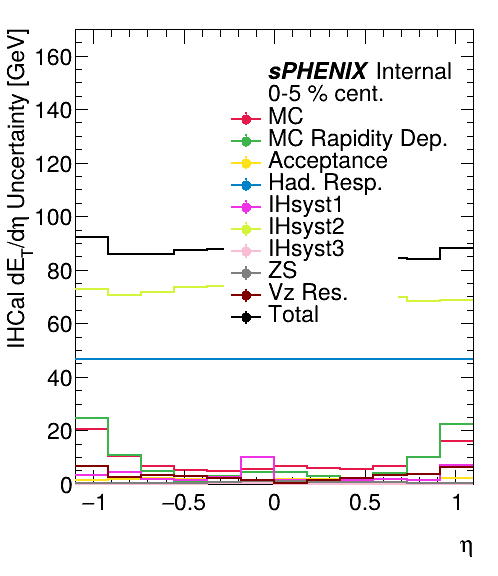
\includegraphics[width=0.32\linewidth]{figures/chapter4/ihcal_total_syst_0-5.png}
    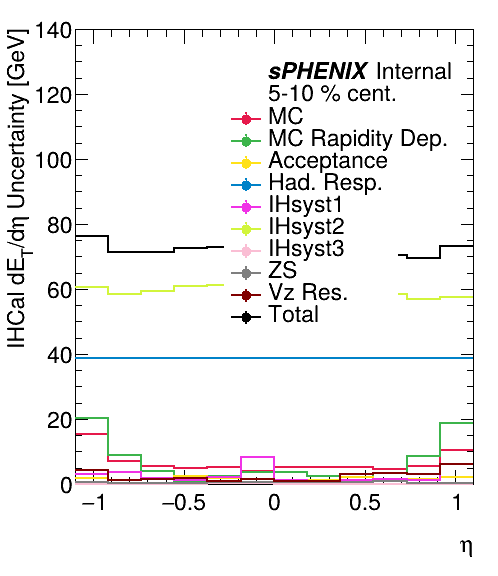
\includegraphics[width=0.32\linewidth]{figures/chapter4/ihcal_total_syst_5-10.png}
    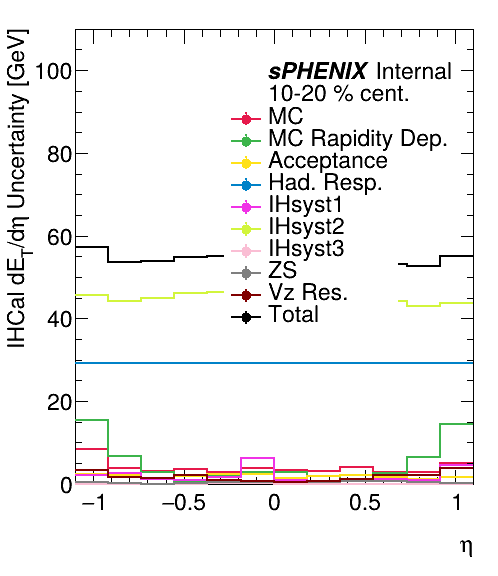
\includegraphics[width=0.32\linewidth]{figures/chapter4/ihcal_total_syst_10-20.png}
    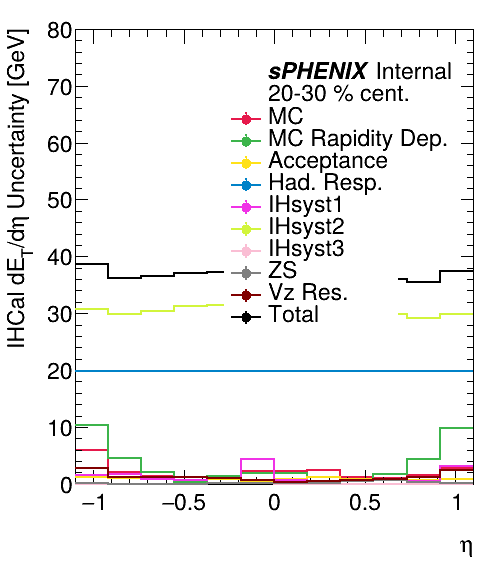
\includegraphics[width=0.32\linewidth]{figures/chapter4/ihcal_total_syst_20-30.png}
    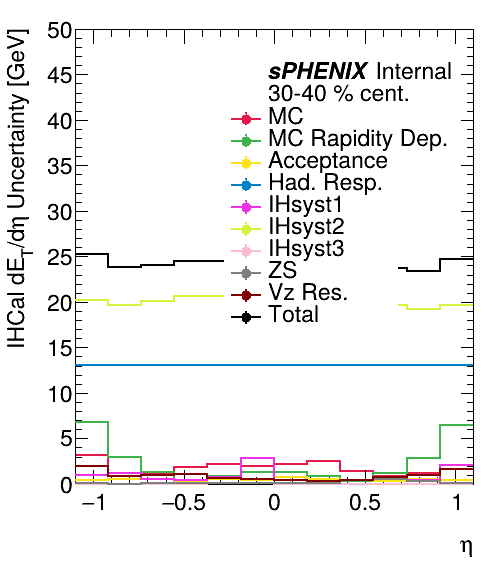
\includegraphics[width=0.32\linewidth]{figures/chapter4/ihcal_total_syst_30-40.png}
    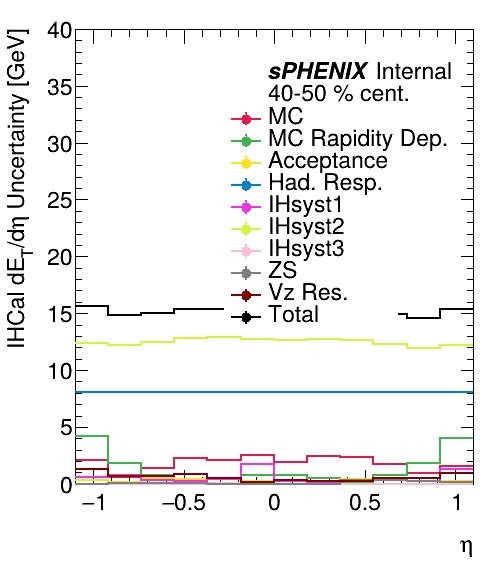
\includegraphics[width=0.32\linewidth]{figures/chapter4/ihcal_total_syst_40-50.png}
    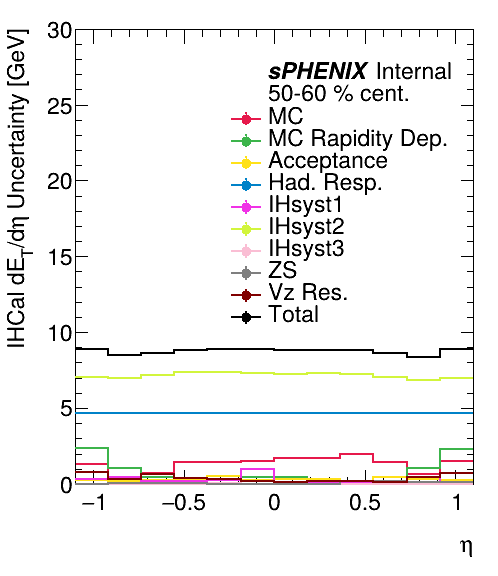
\includegraphics[width=0.32\linewidth]{figures/chapter4/ihcal_total_syst_50-60.png}
    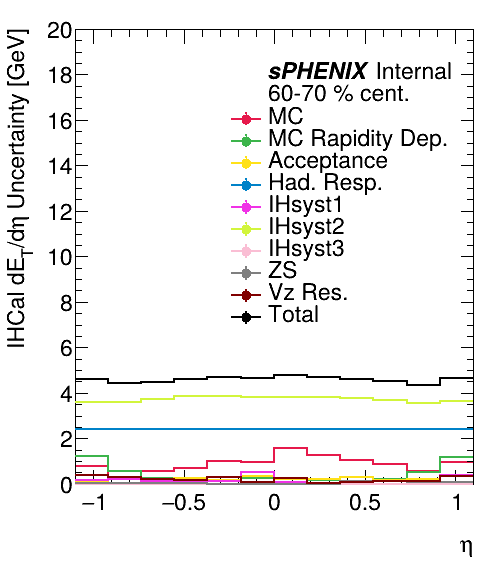
\includegraphics[width=0.32\linewidth]{figures/chapter4/ihcal_total_syst_60-70.png}
    \caption{Systematic uncertainties on \detdeta measurements as a function of $\eta$ for \detdeta measurements from IHCal-only data. Uncertainties from all centralities in measurement are shown in increasing order from top to bottom.}
    \label{fig:eta_dep_syst_ihcal}
\end{figure}

\begin{figure}
    \centering
    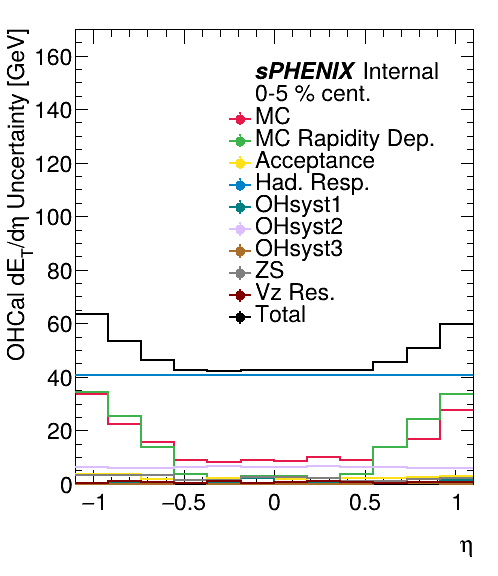
\includegraphics[width=0.32\linewidth]{figures/chapter4/ohcal_total_syst_0-5.png}
    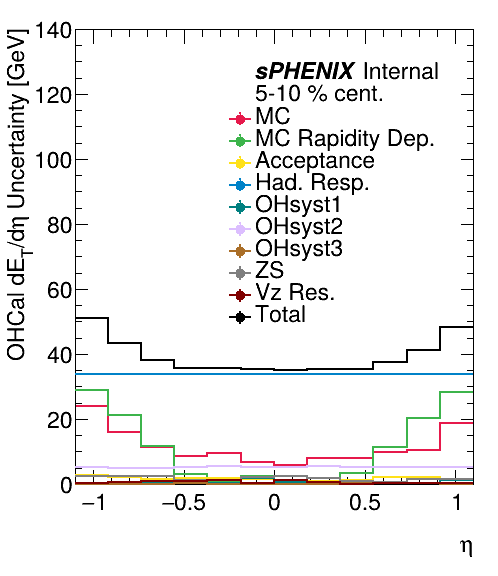
\includegraphics[width=0.32\linewidth]{figures/chapter4/ohcal_total_syst_5-10.png}
    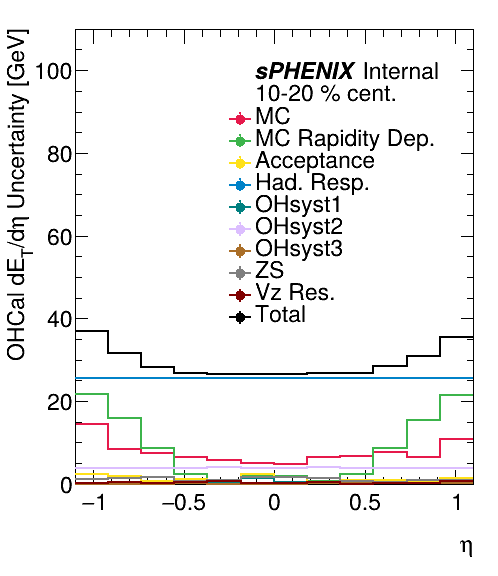
\includegraphics[width=0.32\linewidth]{figures/chapter4/ohcal_total_syst_10-20.png}
    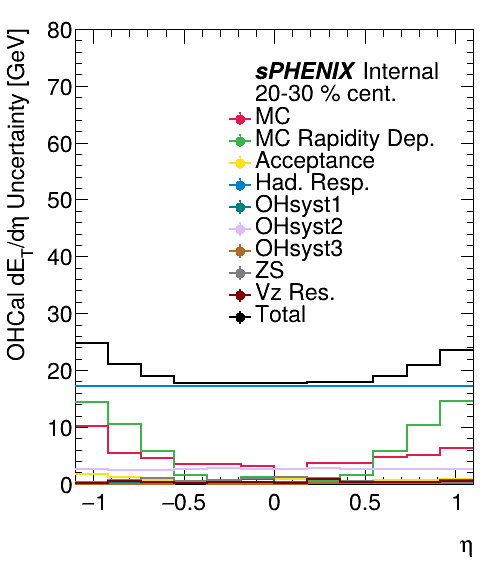
\includegraphics[width=0.32\linewidth]{figures/chapter4/ohcal_total_syst_20-30.png}
    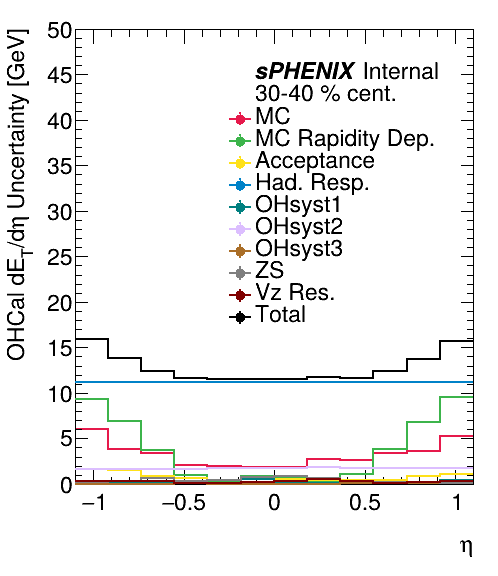
\includegraphics[width=0.32\linewidth]{figures/chapter4/ohcal_total_syst_30-40.png}
    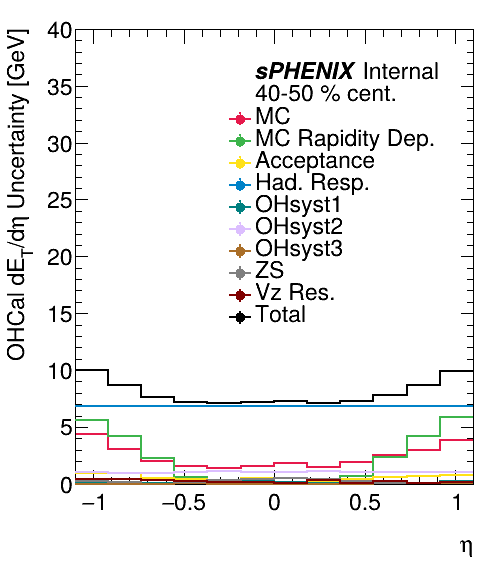
\includegraphics[width=0.32\linewidth]{figures/chapter4/ohcal_total_syst_40-50.png}
    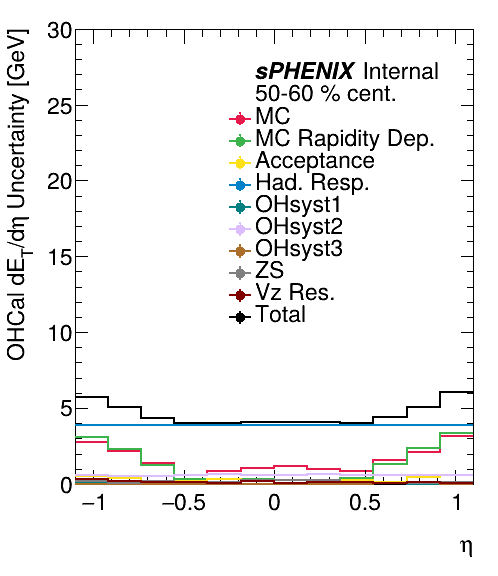
\includegraphics[width=0.32\linewidth]{figures/chapter4/ohcal_total_syst_50-60.png}
    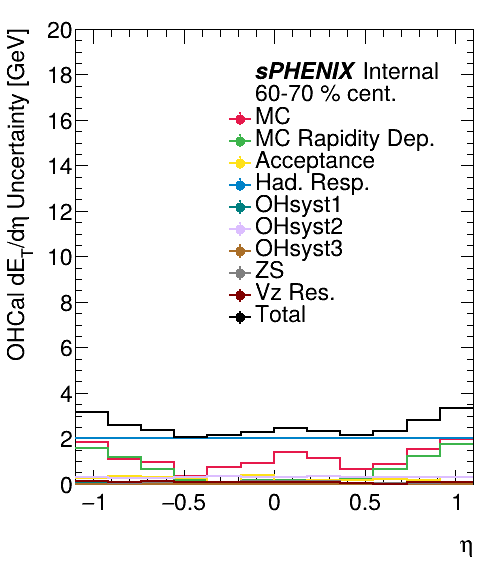
\includegraphics[width=0.32\linewidth]{figures/chapter4/ohcal_total_syst_60-70.png}
    \caption{Systematic uncertainties on \detdeta measurements as a function of $\eta$ for \detdeta measurements from OHCal-only data. Uncertainties from all centralities in measurement are shown in increasing order from top to bottom.}
    \label{fig:eta_dep_syst_ohcal}
\end{figure}

The metholodogy for determining the correlation between \detdeta measurements and finding the agreement between measurements within uncorrelated uncertainties is also outlined in Section~\ref{sec:detdeta_systematics}.
Additional scatter plots for determining the correlation between the positive and negative $\eta$ measurements of \detdeta using only EMCal or HCal data are included in Figures~\ref{fig:emcal_eta_covariance} and \ref{fig:hcal_eta_covariance}.
Finally, the ratio of measurements of \detdeta at positive and negative $\eta$ using only the EMCal or HCal data are included in Figures~\ref{fig:emcal_eta_detdeta_ratio} and \ref{fig:hcal_eta_detdeta_ratio}.

\begin{figure}
    \centering
    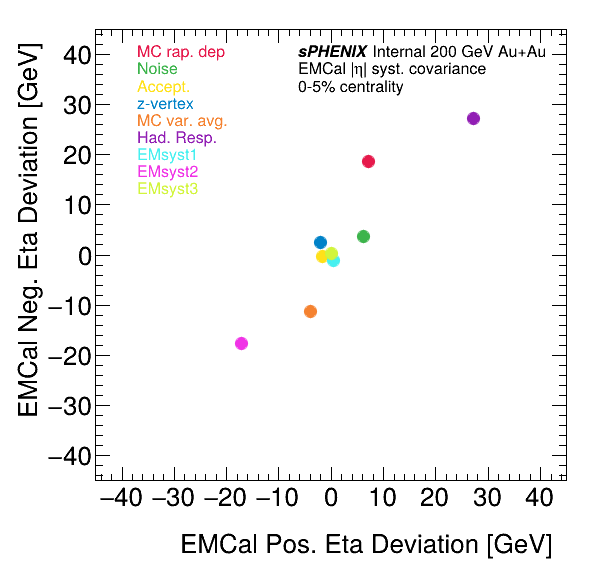
\includegraphics[width=0.32\linewidth]{detdeta/Figures/corr_syst_uncertainties/emcal_pos_neg_eta_covariance_0-5.png}
    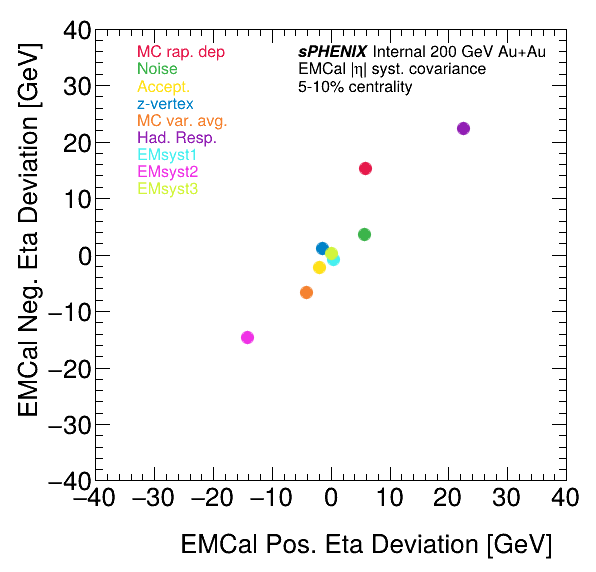
\includegraphics[width=0.32\linewidth]{detdeta/Figures/corr_syst_uncertainties/emcal_pos_neg_eta_covariance_5-10.png}
    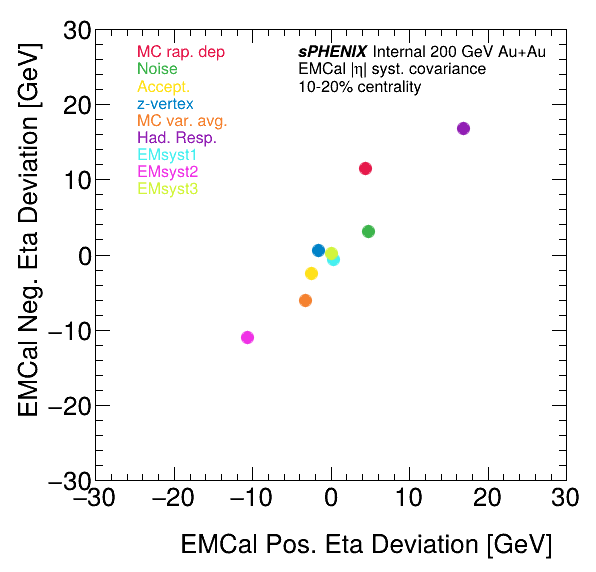
\includegraphics[width=0.32\linewidth]{detdeta/Figures/corr_syst_uncertainties/emcal_pos_neg_eta_covariance_10-20.png}
    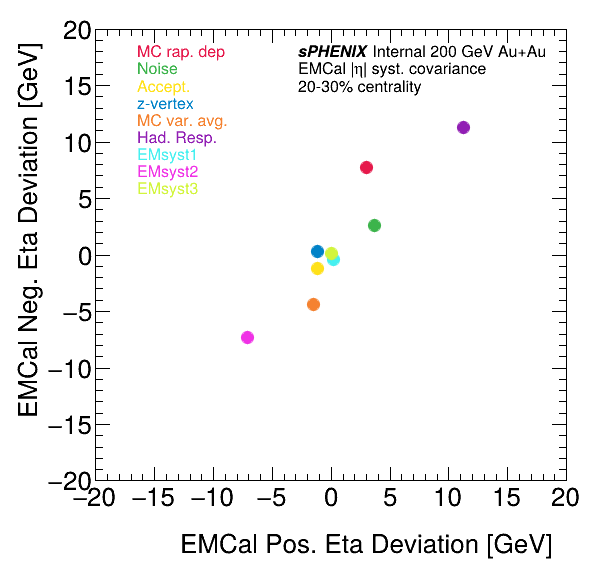
\includegraphics[width=0.32\linewidth]{detdeta/Figures/corr_syst_uncertainties/emcal_pos_neg_eta_covariance_20-30.png}
    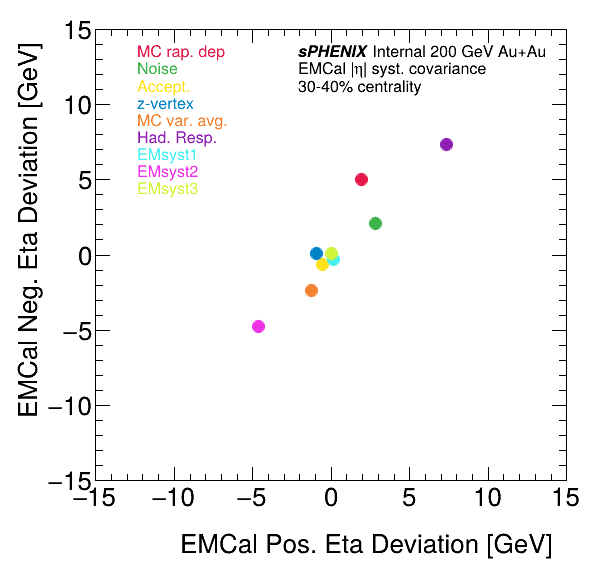
\includegraphics[width=0.32\linewidth]{detdeta/Figures/corr_syst_uncertainties/emcal_pos_neg_eta_covariance_30-40.png}
    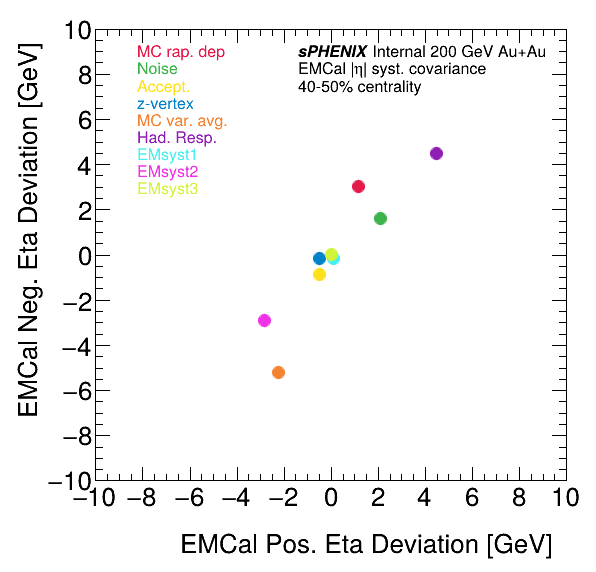
\includegraphics[width=0.32\linewidth]{detdeta/Figures/corr_syst_uncertainties/emcal_pos_neg_eta_covariance_40-50.png}
    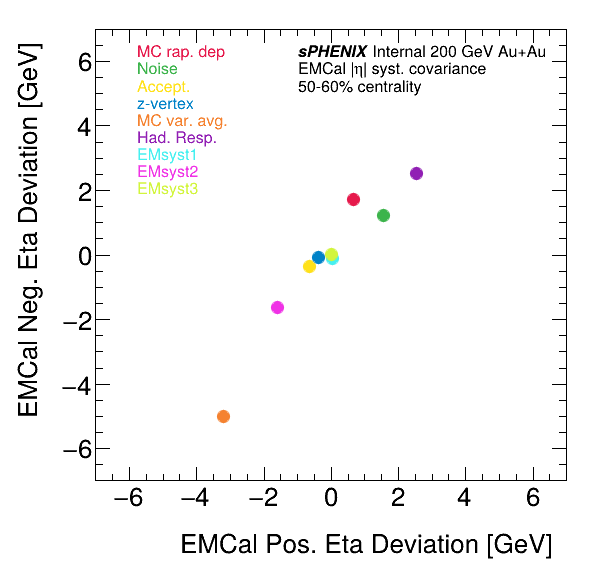
\includegraphics[width=0.32\linewidth]{detdeta/Figures/corr_syst_uncertainties/emcal_pos_neg_eta_covariance_50-60.png}
    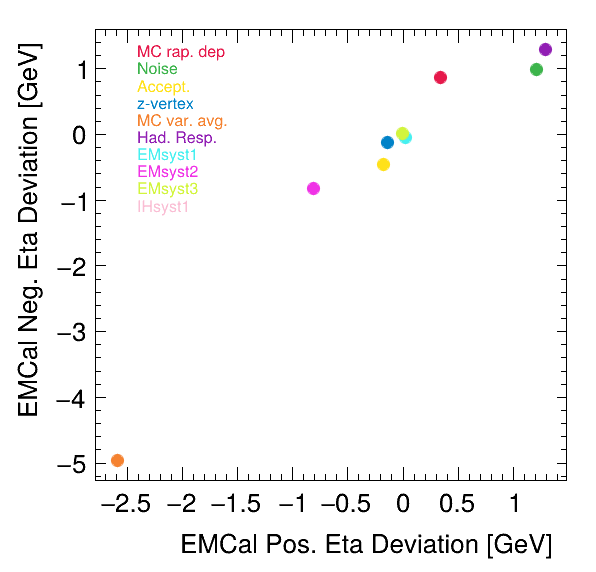
\includegraphics[width=0.32\linewidth]{figures/chapter4/emcal_pos_neg_eta_covariance_prc_edit_60-70.png}
    \caption{Correlation plots for the EMCal \detdeta measurements at $0.74 < |\eta| < 1.1$ using each analysis systematic variation for each centrality measurement in the analysis.}
    \label{fig:emcal_eta_covariance}
\end{figure}
\begin{figure}
    \centering
    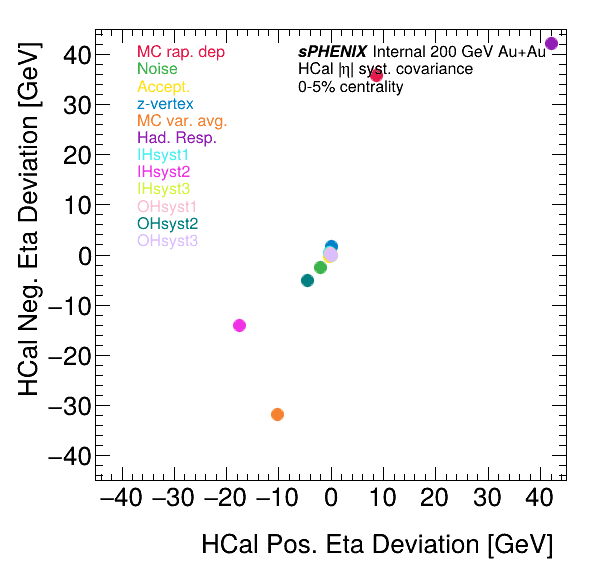
\includegraphics[width=0.32\linewidth]{detdeta/Figures/corr_syst_uncertainties/hcal_pos_neg_eta_covariance_0-5.png}
    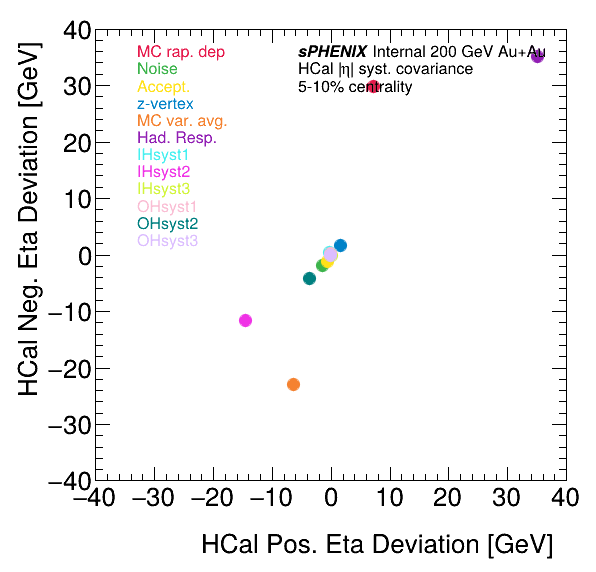
\includegraphics[width=0.32\linewidth]{detdeta/Figures/corr_syst_uncertainties/hcal_pos_neg_eta_covariance_5-10.png}
    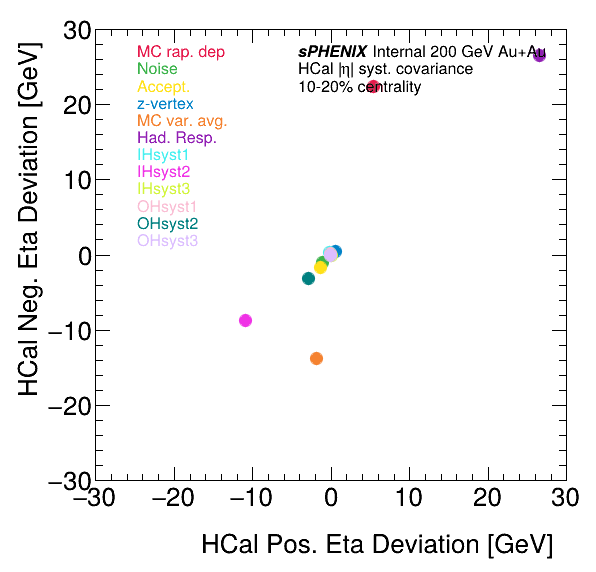
\includegraphics[width=0.32\linewidth]{detdeta/Figures/corr_syst_uncertainties/hcal_pos_neg_eta_covariance_10-20.png}
    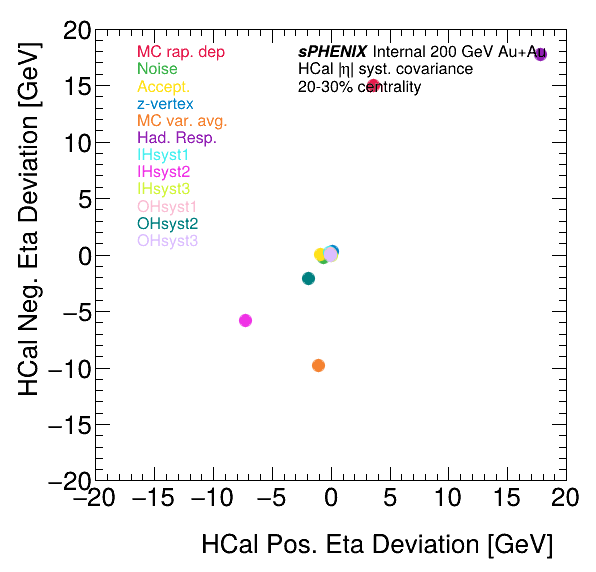
\includegraphics[width=0.32\linewidth]{detdeta/Figures/corr_syst_uncertainties/hcal_pos_neg_eta_covariance_20-30.png}
    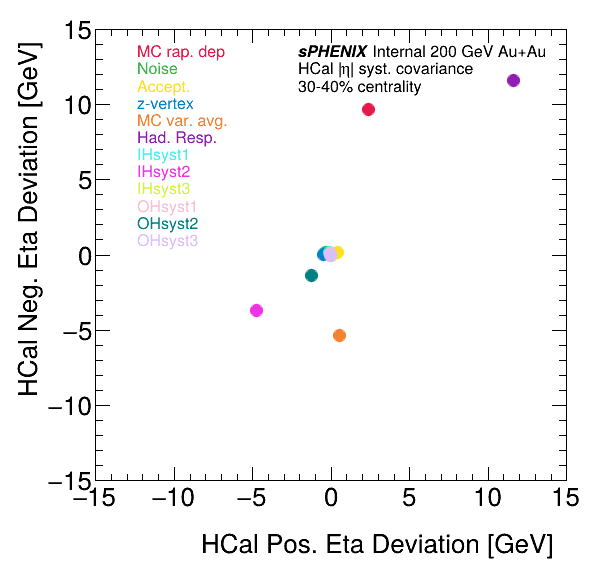
\includegraphics[width=0.32\linewidth]{detdeta/Figures/corr_syst_uncertainties/hcal_pos_neg_eta_covariance_30-40.png}
    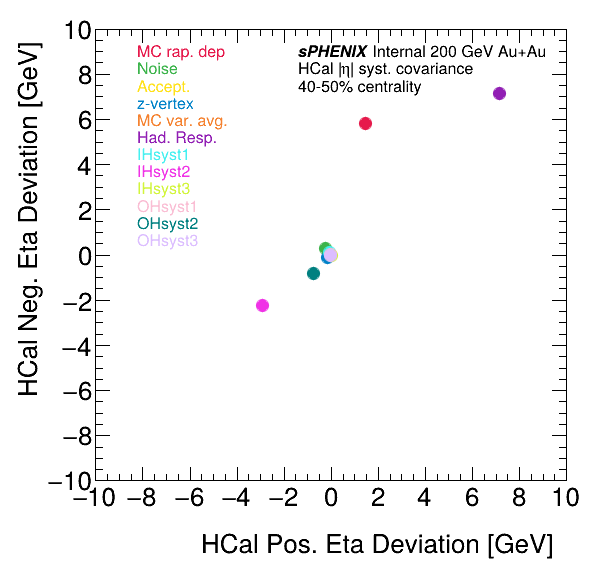
\includegraphics[width=0.32\linewidth]{detdeta/Figures/corr_syst_uncertainties/hcal_pos_neg_eta_covariance_40-50.png}
    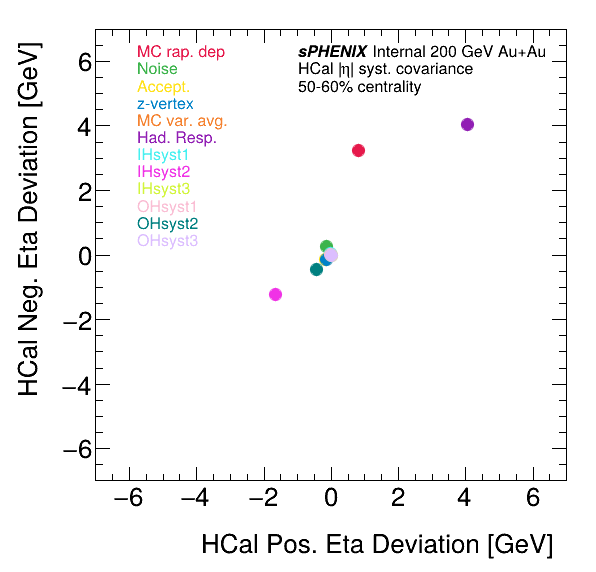
\includegraphics[width=0.32\linewidth]{detdeta/Figures/corr_syst_uncertainties/hcal_pos_neg_eta_covariance_50-60.png}
    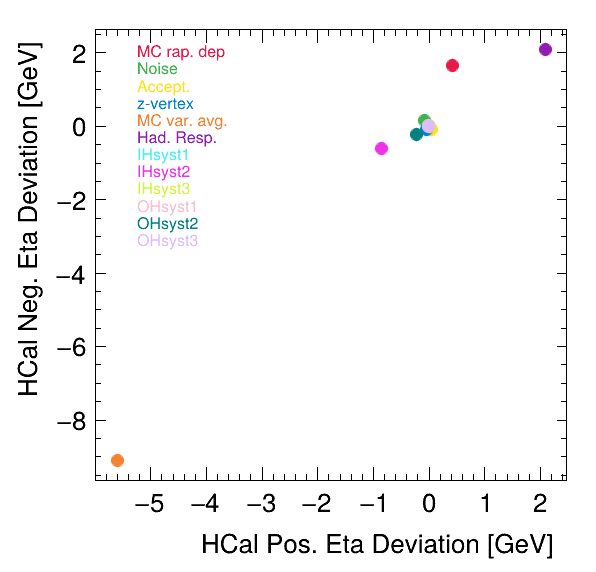
\includegraphics[width=0.32\linewidth]{figures/chapter4/hcal_pos_neg_eta_covariance_prc_edit_60-70.png}
    \caption{Correlation plots for the HCal \detdeta measurements at $0.74 < |\eta| < 1.1$ using each analysis systematic variation for each centrality measurement in the analysis.}
    \label{fig:hcal_eta_covariance}
\end{figure}

\begin{figure}
    \centering
    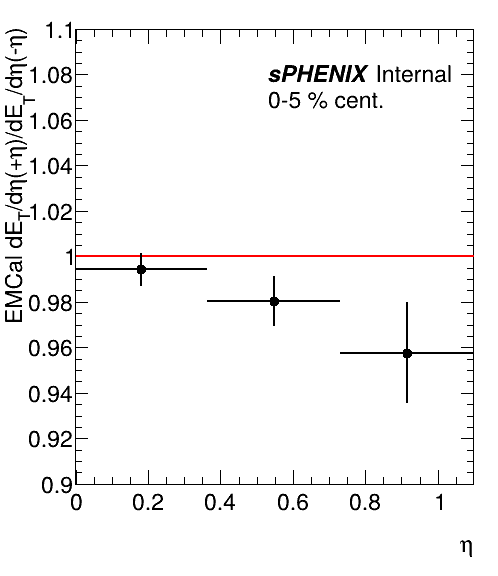
\includegraphics[width=0.32\linewidth]{detdeta/Figures/corr_syst_uncertainties/emcal_eta_ratio_syst_0-5.png}
    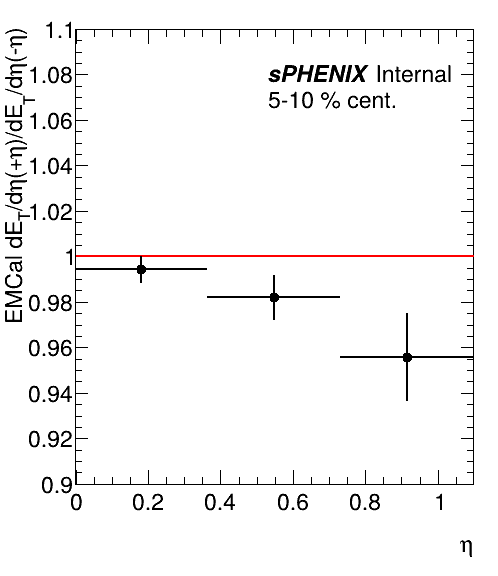
\includegraphics[width=0.32\linewidth]{detdeta/Figures/corr_syst_uncertainties/emcal_eta_ratio_syst_5-10.png}
    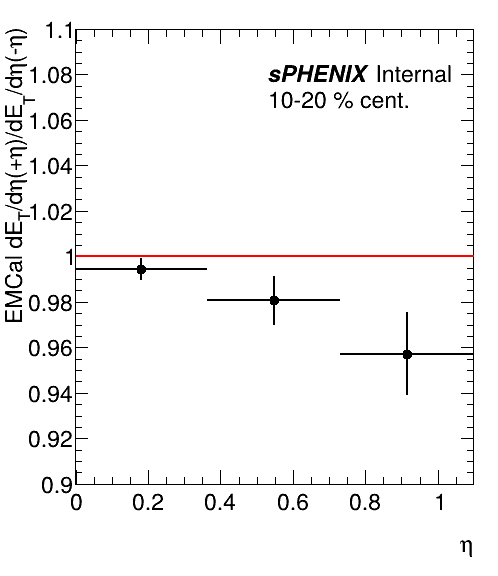
\includegraphics[width=0.32\linewidth]{detdeta/Figures/corr_syst_uncertainties/emcal_eta_ratio_syst_10-20.png}
    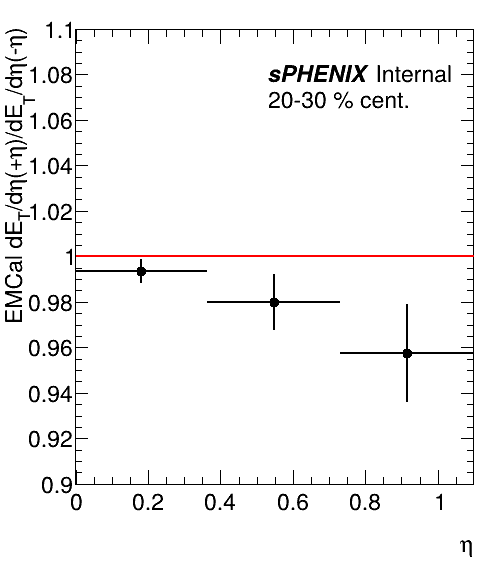
\includegraphics[width=0.32\linewidth]{detdeta/Figures/corr_syst_uncertainties/emcal_eta_ratio_syst_20-30.png}
    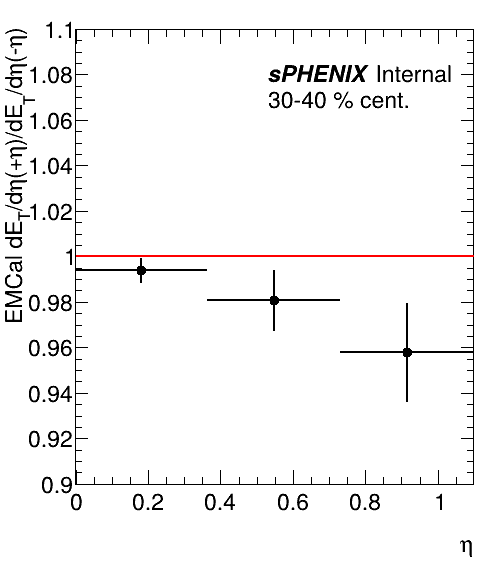
\includegraphics[width=0.32\linewidth]{detdeta/Figures/corr_syst_uncertainties/emcal_eta_ratio_syst_30-40.png}
    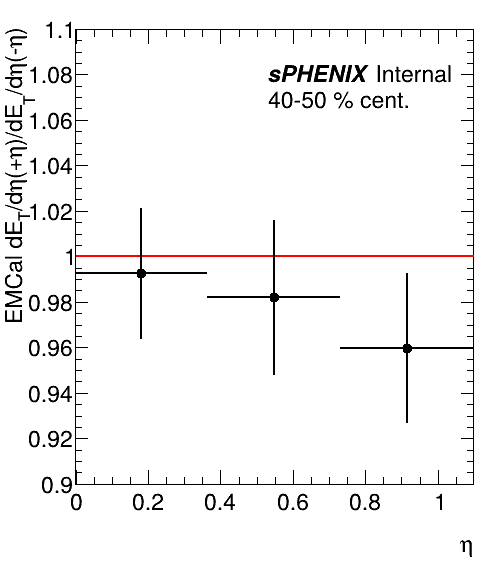
\includegraphics[width=0.32\linewidth]{detdeta/Figures/corr_syst_uncertainties/emcal_eta_ratio_syst_40-50.png}
    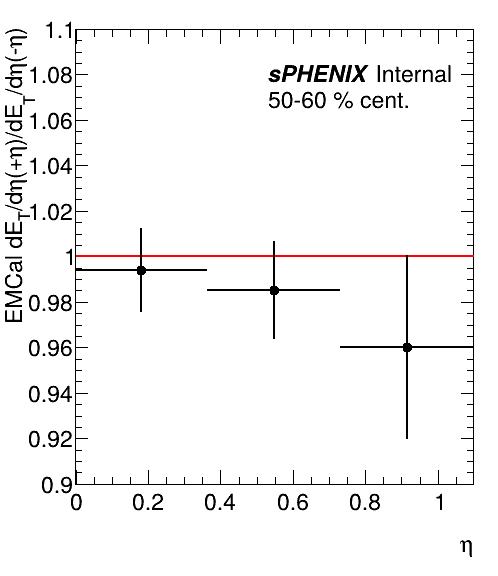
\includegraphics[width=0.32\linewidth]{detdeta/Figures/corr_syst_uncertainties/emcal_eta_ratio_syst_50-60.png}
    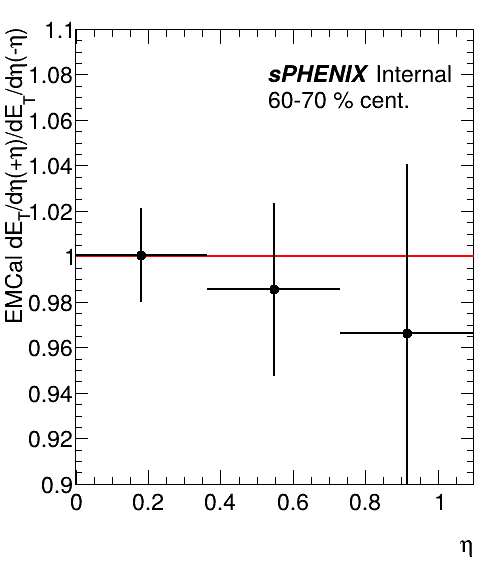
\includegraphics[width=0.32\linewidth]{figures/chapter4/emcal_eta_ratio_syst_60-70.png}
    \caption{Correlation plots for the EMCal \detdeta measurements at $0.74 < |\eta| < 1.1$ using each analysis systematic variation for each centrality measurement in the analysis.}
    \label{fig:emcal_eta_detdeta_ratio}
\end{figure}
\begin{figure}
    \centering
    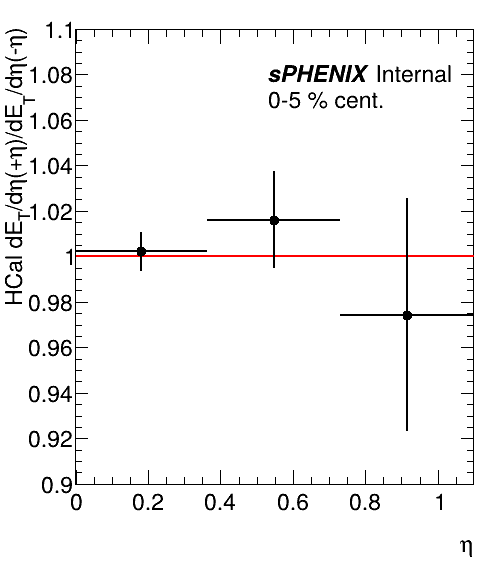
\includegraphics[width=0.32\linewidth] {detdeta/Figures/corr_syst_uncertainties/hcal_eta_ratio_syst_0-5.png}
    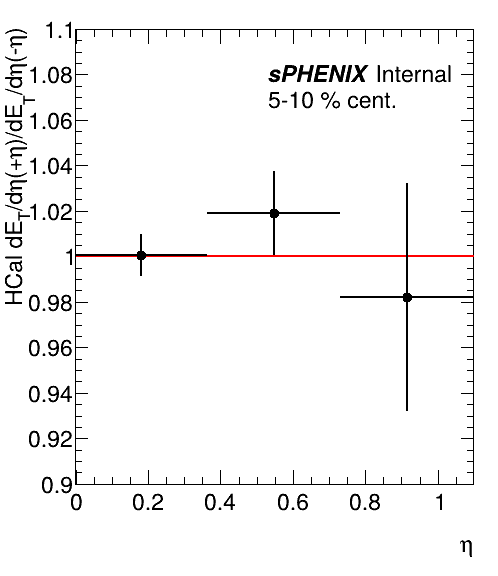
\includegraphics[width=0.32\linewidth]{detdeta/Figures/corr_syst_uncertainties/hcal_eta_ratio_syst_5-10.png}
    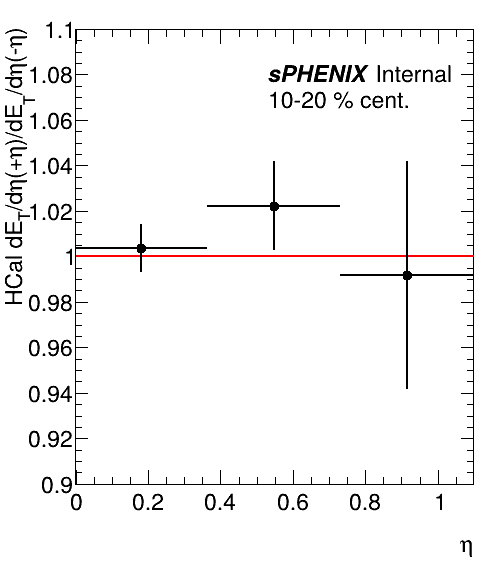
\includegraphics[width=0.32\linewidth]{detdeta/Figures/corr_syst_uncertainties/hcal_eta_ratio_syst_10-20.png}
    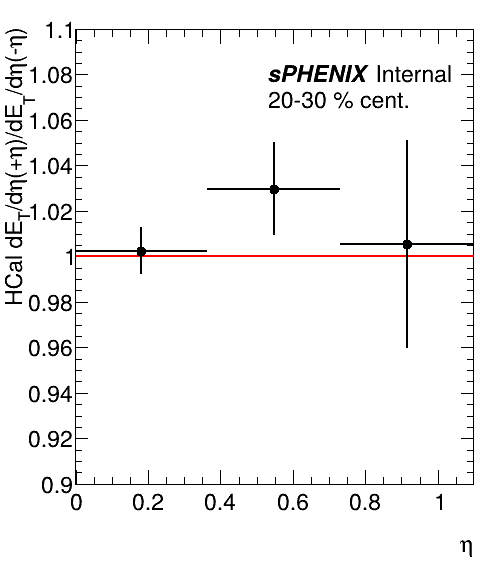
\includegraphics[width=0.32\linewidth]{detdeta/Figures/corr_syst_uncertainties/hcal_eta_ratio_syst_20-30.png}
    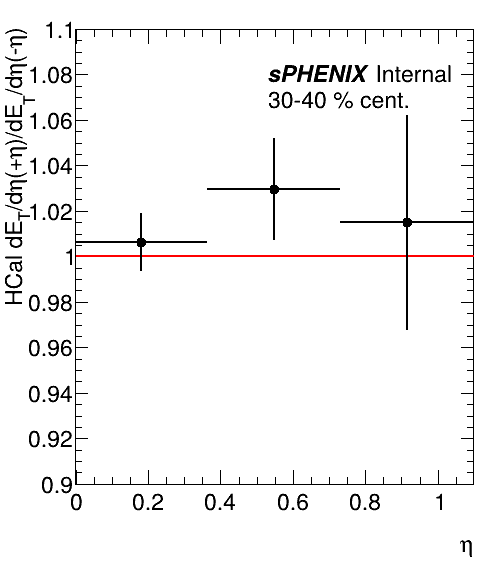
\includegraphics[width=0.32\linewidth]{detdeta/Figures/corr_syst_uncertainties/hcal_eta_ratio_syst_30-40.png}
    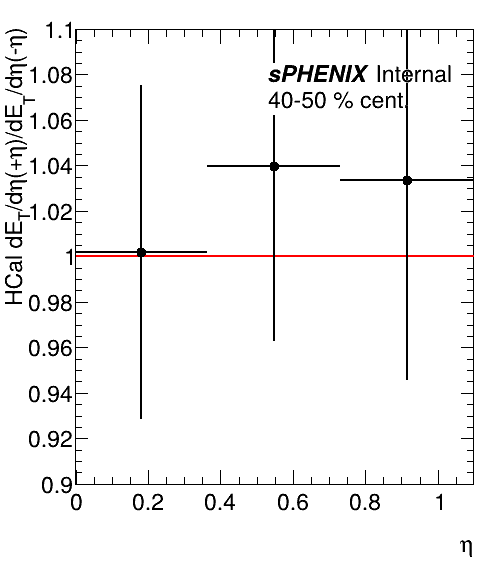
\includegraphics[width=0.32\linewidth]{detdeta/Figures/corr_syst_uncertainties/hcal_eta_ratio_syst_40-50.png}
    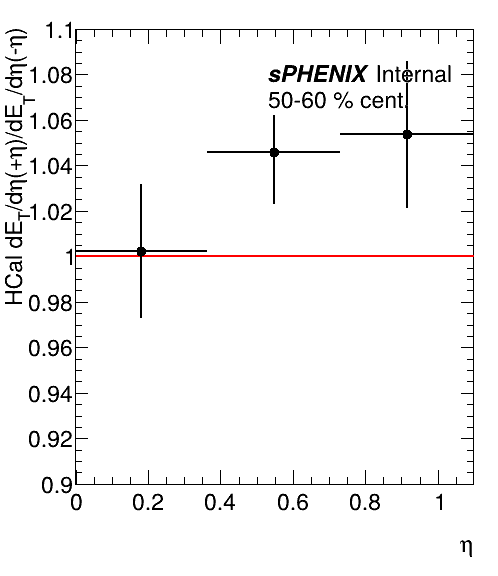
\includegraphics[width=0.32\linewidth]{detdeta/Figures/corr_syst_uncertainties/hcal_eta_ratio_syst_50-60.png}
    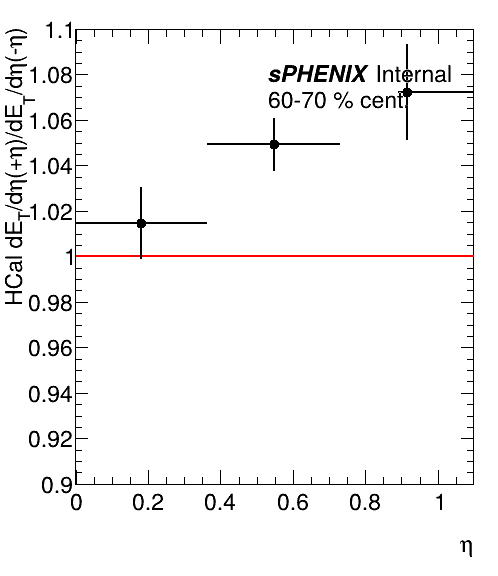
\includegraphics[width=0.32\linewidth]{figures/chapter4/hcal_eta_ratio_syst_60-70.png}
    \caption{Correlation plots for the HCal \detdeta measurements at $0.74 < |\eta| < 1.1$ using each analysis systematic variation for each centrality measurement in the analysis.}
    \label{fig:hcal_eta_detdeta_ratio}
\end{figure}